\section{Basic principles} \label{sec:basic_filter}
A digital filter is characterised as an LTI system, previously defined by equation \eqref{eq:LTI_diff_equation_finite}. As described the system is completely characterized by its corresponding impulse response $h[n]$. In terms of the LTI system as a filter the output $y[n]$ is the part of the signal that comes through the filter. \\
$y[n]$ was previous defined by \eqref{def:convolution} as the convolution sum of input signal and impulse response of the system
\begin{align}
y[n] = x[n]*h[n] = \sum_{k=-\infty}^{\infty} x[k]h[n-k].
\end{align}    
The frequency response of the system is given by the Fourier transform of the impulse response - analogue to definition \ref{def:Fourier_trans} for a discrete sequence - as
\begin{align}\label{eq:freq_res}
H(\omega)=\sum_{k=-\infty}^{\infty}h[k]e^{-j\omega k}.
\end{align}
It is known from the definition that $H(\omega)$ can be expressed as
\begin{align}
H(\omega)=|H(\omega)|e^{j\measuredangle H(\omega)},
\end{align}  
where $|H(\omega)|$ and $e^{j\measuredangle H(\omega)}$ are the \textit{amplitude} and \textit{phase} response of the filter respectively, both real valued and $2\pi$-periodic.\\
If $H(\omega)$ is real it is said to have \textit{zero phase}, which is equivalent to the phase response only taking values that are integer multiples of $\pi$, resulting in a straight phase with zero slope. Further if $H(\omega)$ can be written in the form 
\begin{align}\label{eq:lin_pha}
H(\omega)=A(\omega)e^{j(-\alpha\omega + j\beta)} ,
\end{align}
where $\alpha$ and $\beta$ are constants and $A(\omega)$ is real, the filter is said to have \textit{general linear phase}. That is because the phase response consists of constant terms added to the linear function making a straight line with slope $\alpha$ except from the discontinuities resulting from jumps of $2\pi$ caused by the $2\pi$-periodicity. \\
A generalized linear phase response is characterized by a constant \textit{group delay} $\tau(\omega)$:
\begin{align}
\tau(\omega)=-\frac{d}{d\omega}\left\{ \measuredangle H(\text{e}^{j\omega} \right\} = \alpha.
\end{align}
The phase response is an expression of how each of the signal components are delayed though the system, where linear phase indicates an equal delay for all components of the signal. To guarantee a constant group delay, $\alpha$, $\beta$ and $h[n]$ has to fulfil the following condition, for all $\omega$ \cite{DTSP, page 341}
\begin{align}\label{eq:cons_gro}
\sum_{n=-\infty}^{\infty}h[n]\sin\left(\omega \left(n-\alpha \right) + \beta \right) = 0.
\end{align}

\subsection{Ideal filters} \label{sec:ideal_filt}
When designing filters it is ideal to have constant amplitude and zero phase corresponding to the frequency response. \\ For an ideal selective frequency filter the amplitude response will be constant unity for the frequencies that are wanted to pass the filter referred to as the \textit{bandpass} and zero for all other frequencies referred to as \textit{bandstop}. An example is an ideal lowpass filter with frequency response 
\begin{align}\label{eq:low}
H_{lp}(\omega)=
\left\{ \begin{matrix}
1, &\ \left| \omega \right|< \omega_c \\
0, &\ \omega_c < \left| \omega \right| \leq \pi
\end{matrix}\right.,
\end{align}     
where $H_{lp}(\omega)$ is $2\pi$ periodic. $\omega_c$ is referred to as the \textit{cutoff frequency}. The lowpass filter selects the frequencies lower than the cutoff frequency and reject the higher frequency components of the input signal. By \eqref{eq:low} it is seen that the lowpass filter is real valued hence has zero phase as expected. \\
The corresponding impulse response are determined by the inverse Fourier transform on the passband interval - analogue to definition \ref{def:InverseFourier_trans} for a discrete sequence.
\begin{align}\label{eq:low_im}
h_{lp}[n]= \frac{1}{2\pi}\int_{-\pi}^{\pi}\text{e}^{j\omega n} d\omega =\frac{1}{2\pi}\int_{-\omega_c}^{\omega_c}\text{e}^{j\omega n} d\omega = \frac{1}{2\pi j n}\left[\text{e}^{j\omega n} \right]_{-\omega_c}^{\omega_c} = \frac{\sin \omega_c n}{\pi n }, \ \  -\infty < n < \infty.
\end{align} 
Note that the first equality is true because by \eqref{eq:low} the integral is zero outside the interval $[-\omega_c, \omega_c]$. \eqref{eq:low} is only true for $n \neq 0$ and $h_{lp}[0]$ must be defined separately. For this l'Hôspitals rule $\lim \frac{f(x)}{g(x)}=\lim \frac{f'(x)}{g'(x)}$ is used. Thus
\begin{align}
h_{lp}[0]=& \frac{1}{\pi} \left( \cos\left( \omega_{c} n \right)\omega_{c}\right)
= \frac{1}{\pi}\left( \omega_{c} \right).
\end{align}

By \eqref{eq:low_im} the impulse response is non-zero for all $n<0$ thus the filter is non-casual according to definition \ref{def:causal_system}.\\
Amplitude- and impulse response of the ideal lowpass filter are illustrated on figure \ref{fig:ideal_low}
\begin{figure}[H]
\begin{subfigure}[b]{0.50\textwidth}
        \centering
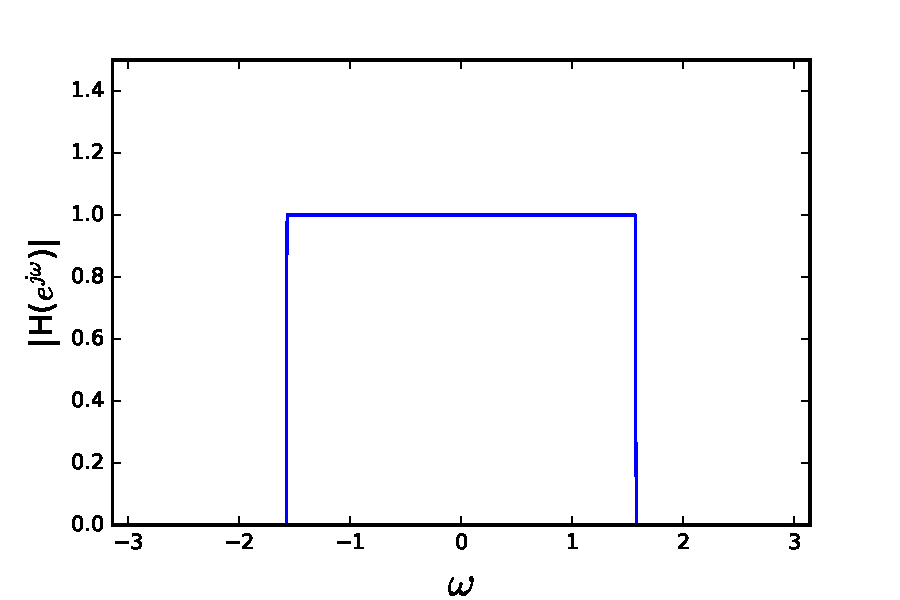
\includegraphics[scale=0.45]{figures/filter_teori/ideal_low2.pdf}
\caption{}
\end{subfigure}
\begin{subfigure}[b]{0.50\textwidth}
        \centering  
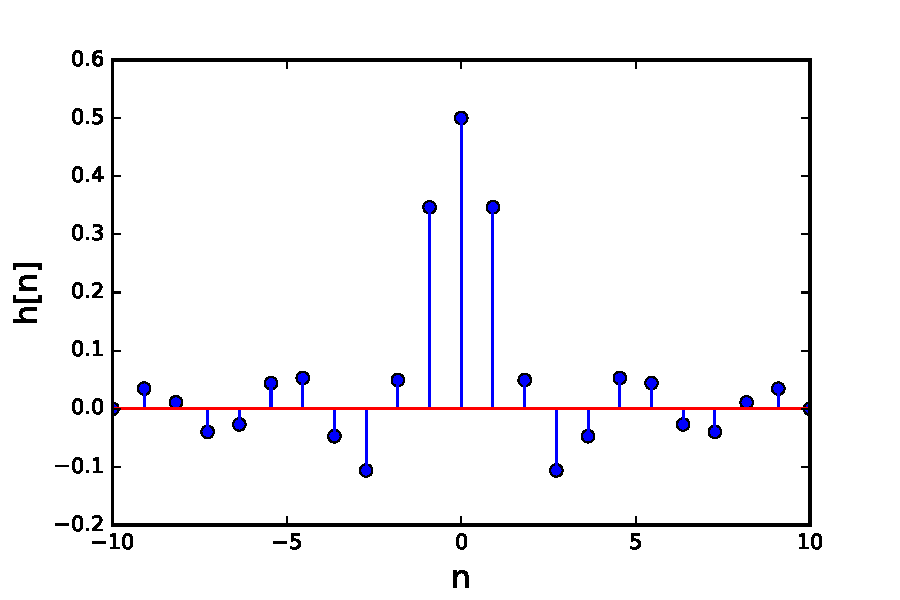
\includegraphics[scale=0.45]{figures/filter_teori/ideal_low1.pdf}
\caption{}
 \end{subfigure}
\caption{ (a) Amplitude response of ideal lowpass filter with $\omega_c = \frac{\pi}{2}$ (b) corresponding impulse response}
\label{fig:ideal_low}
\end{figure}


Analogues of ideal highpass or bandpass filter can be defined, as illustrated on figure \ref{fig:ideal}.\\ 

\begin{figure}[H]
\begin{subfigure}[b]{0.50\textwidth}
        \centering
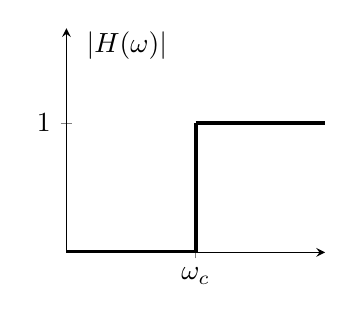
\begin{tikzpicture}[scale=1]
\begin{axis}[
scale=0.5,
unit vector ratio*=1 1 1,
axis lines = middle,
xtick={1.5},
xticklabels={$\omega_c$},
ytick={1.5},
yticklabels={$1$},
xmin=0,
xmax=3,
ymin=0,
ymax=2.6]
\node at (axis cs:0.7,2.4) {$|H(\omega)|$};
\draw[line width=0.6mm](axis cs:0,0)--(axis cs:1.5,0);
\draw[line width=0.5mm](axis cs:1.5,1.5)--(axis cs:3,1.5);
\draw[line width=0.5mm](axis cs:1.5,1.5)--(axis cs:1.5,0);
\end{axis}
\end{tikzpicture}

\caption{}
    \end{subfigure}
 \begin{subfigure}[b]{0.50\textwidth}
        \centering  
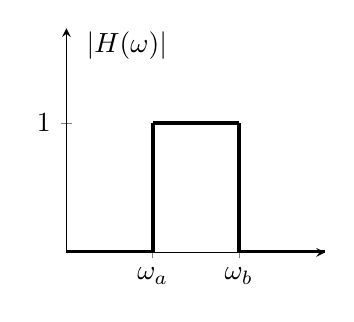
\begin{tikzpicture}[scale=1]
\begin{axis}[
scale=0.5,
unit vector ratio*=1 1 1,
axis lines = middle,
xtick={1,2},
xticklabels={$\omega_a$,$\omega_b$},
ytick={1.5},
yticklabels={$1$},
xmin=0,
xmax=3,
ymin=0,
ymax=2.6]
\node at (axis cs:0.7,2.4) {$|H(\omega)|$};
\draw[line width=0.5mm](axis cs:1,1.5)--(axis cs:1,0);
\draw[line width=0.5mm](axis cs:1,1.5)--(axis cs:2,1.5);
\draw[line width=0.5mm](axis cs:2,1.5)--(axis cs:2,0);
\draw[line width=0.5mm](axis cs:1,0)--(axis cs:0,0);
\draw[line width=0.5mm](axis cs:2,0)--(axis cs:3,0);
\end{axis}
\end{tikzpicture}
\caption{}
    \end{subfigure}
\caption{Amplitude response of ideal (a) highpass filter (B) bandpass filter}
\label{fig:ideal}
\end{figure}
As stated in section \ref{sec:LTI} a non-causal LTI system is not realizable. Furthermore  zero phase is not possible for a causal system.
Thus an approximation of an ideal filter can be computed by a casual system with general linear phase.    

\section{FIR and IIR filter} 
Two classes of filter are essential to identify.
For all ideal filters discussed in the previous section the impulse response is defined for $-\infty < n < \infty$. Such a filter is specified as an \textit{infinite impulse response (IIR)} filter. In the case of the impulse response being zero outside a finite interval the filter is referred to as a \textit{finite impulse response (FIR)} filter. 
\subsection{Type 1 FIR filter}
As described causal systems with generalized linear phase is a possible approximation of the ideal filter. This is to be guaranteed by using specific types of FIR filters.\\
A causal system with generalized linear phase has to fulfil the following relation, cf. section \ref{sec:basic_filter}:
\begin{align}
\sum_{n=0}^{\infty}h[n]\sin\left(\omega \left(n-\alpha \right) + \beta \right) = 0
\end{align}
For a FIR filter to satisfy this relation the following set of conditions has to be fulfilled \cite{DTSP, p.342}:
\begin{align} \label{eq:FIR_con}
&\beta = \left\{ \begin{matrix} 
\pi  \\
0 
\end{matrix}\right. \nonumber  \\ 
&2\alpha = M = \text{an integer} \\ 
&h[n]=h[M-n] \ \text{or} \ h[n]=-h[M-n]. \nonumber  
\end{align} 
This implies that $h[n]$ is either symmetric or anti symmetric and that $\alpha = \frac{M}{2}$ becomes the symmetry point. \\
From these conditions four different types of FIR filter with generalized linear phase are defined \cite{DTSP, page 343}, only the \textit{type 1 FIR filter} will be elaborated here.
A type 1 FIR filter is characterised by having a symmetric impulse response and $M$ being an even integer. By applying the symmetry condition to the definition of the Fourier transform $H(\omega)$ is defined as \cite{page 343,DTSP}   
\begin{align}\label{eq:type1}
H(\omega)=\text{e}^{-j\omega \frac{M}{2}} \sum_{k=0}^{\frac{M}{2}} a[k]\cos \omega k,
\end{align}
where 
\begin{align}
a[k]= \left\{ \begin{matrix}
2h\left[ \frac{M}{2} - k \right], \ \ &\ k=1,2,... , \frac{M}{2}.   \\
h[\frac{M}{2}], \ \ &\ k = 0  
\end{matrix}\right.
\end{align}
By this \eqref{eq:type1} has the form of \eqref{eq:lin_pha} where $A(\omega)= \sum_{k=0}^{\frac{M}{2}} a[k]\cos \omega k$ is a real function of $\omega$ and $\beta$ equals either 0 or $\pi$. Hence a constant group delay is achieved.








   
 


 



